%\subsection{Tablero}
%Sobre él se juegan las partidas, tiene implementadas tanto las reglas del juego tradicional, como las reglas de la mecánica cuántica para volver de este un juego más interesante. Además ya contiene el tablero y las piezas necesarias para poder desarrollar todas las simulaciones posibles, y además que pueda ser jugado por una persona normal. Los movimientos especiales con mecánica cuántica que se emplearon son los siguientes:

\section{Metodología}

Con el fin de poder jugar de manera correcta, coherente y desafiante al ajedrez cuántico; se requiere el uso de una red neuronal que pueda ser capaz de calcular movimientos a partir de un estado inicial. Dicho estado es un tablero común y corriente con las piezas en él. Para poder llegar a este objetivo se ha planteado el siguiente gráfico que representa el pipeline por el cual se conseguirá la data, para posteriormente usarse en el entrenamiento de la red neuronal, y también tener en cuenta el ajuste de hiper parámetros mediante un algoritmo metaheurístico.

\begin{center}
	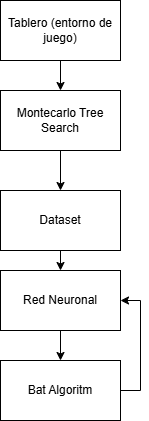
\includegraphics[scale=0.5] {Imagenes/Trabajo_RED_NEURONAL.drawio.png}
\end{center}

A continuación una breve descripción de cada componente del pipeline.

\subsection{Quantum chess}

Sobre él se juegan las partidas, tiene implementadas tanto las reglas del juego tradicional, como las reglas de la mecánica cuántica para volver de este un juego más interesante. Además ya contiene el tablero y las piezas necesarias para poder desarrollar todas las simulaciones posibles, y además que pueda ser jugado por una persona normal.
Los movimientos especiales con mecánica cuántica que se emplearon son los siguientes:

\subsubsection{Movimiento}

Para poder trabajar el movimiento convencional que implica cambiar la posición de una pieza entera, o una superposición de esta misma, a otra; se utilizó la compuerta iSWAP, que se debe aplicar entre los dos qubits que intercambiarán valores.
Esta compuerta lo que hace es intercambiar el valor de un qubit con otro a la hora de colapsar el circuito completo. Y esto sucede por la matriz que representa a la compuerta matemáticamente.

\[
U_{iSwap} = \begin{pmatrix}
	1 & 0 & 0 & 0 \\
	0 & 0 & i & 0 \\
	0 & i & 0 & 0 \\
	0 & 0 & 0 & 1
\end{pmatrix}
\]

Se utiliza esta porque es más sensible a los patrones de memoria y puede aprender de manera más segura los patrones del circuito y así se evitan swaps inefectivos que dejarían el juego injugable por la aleatoriedad.

\subsubsection{Split} 

Para poder realizar una superposición entre dos posiciones, se debe de mantener el uso de la compuerta previamente analizada, pero esto sería únicamente para uno de los dos destinos que implican el split. El otro destino debe verse evaluado mediante sqrt(iSWAP), entre este y el mismo origen.
Esta raíz sobre la compuerta, efectúa una superposición que implica que más adelante cuando se realice el colapso, existirán un 0.5 de probabilidades que aparezca en una posición u otra. Cuantos más splits haya, se irán reduciendo las probabilidades de manera lineal al respecto de cada split o slide realizado.

\[
U_{\sqrt{i\text{SWAP}}} = \begin{pmatrix}
	1 & 0 & 0 & 0 \\
	0 & \frac{1}{\sqrt{2}} & \frac{i}{\sqrt{2}} & 0 \\
	0 & \frac{i}{\sqrt{2}} & \frac{1}{\sqrt{2}} & 0 \\
	0 & 0 & 0 & 1
\end{pmatrix}
\]

\subsubsection{Slide}

El slide implica que se realice un movimiento atravesando a una pieza y pasando sobre ella como si no estuviera. Para poder hacer uso de esta regla, la pieza que será obviada, debe de encontrarse en alguna superposición. Y la compuerta que maneja este proceso, es el Controlled-iSWAP, y se tendrá que aplicar como controlador a la casilla que será atravesada, para sí en caso sea cero se tome en cuenta ese movimiento como válido, mientras que se la pieza controladora se mantuvo ahí al colapsar; el movimiento se invalide por completo.

\[
U_{\text{slide}} = \begin{pmatrix}
	1 & 0 & 0 & 0 & 0 & 0 & 0 & 0 \\
	0 & 0 & i & 0 & 0 & 0 & 0 & 0 \\
	0 & i & 0 & 0 & 0 & 0 & 0 & 0 \\
	0 & 0 & 0 & 1 & 0 & 0 & 0 & 0 \\
	0 & 0 & 0 & 0 & 1 & 0 & 0 & 0 \\
	0 & 0 & 0 & 0 & 0 & 1 & 0 & 0 \\
	0 & 0 & 0 & 0 & 0 & 0 & 1 & 0 \\
	0 & 0 & 0 & 0 & 0 & 0 & 0 & 1 \\
\end{pmatrix}
\]

\subsubsection{Split-Slide}

Para poder realizar un split-slide se optó por utilizar una combinación de compuertas. Es decir, se realizará un Controlled-iSWAP entre la posición y su destino con slide. Para luego en caso ya no hay otro slide, se realice un sqrt(iSWAP) hacia la dirección sin mayor problemas. En caso, sea un slide en la misma dirección, se realice un sqrt(iSWAP), pero tomando como inicio el qubit donde se realizó inicialmente el Controlled-iSWAP. Y por último caso, en caso se vaya a don direcciones distintas y ambos requieren slide, a la segunda se le realizará un sqrt(Controlled-iSWAP) desde el mismo qubit de origen.

\subsubsection{Merge}

Solo es un movimiento que a nivel de lógica permite que se encuentre en esa posición, mas no a nivel matemático, porque luego cuando se realice el colapso, el circuito generado simulará todo y como ese resultado comenzó a moverse junto, no importa de donde llegue, lo que importa es que por un lado, u otro, se mantendrá el camino. Pero la compuerta utilizada será un Controlled-iSWAP para que si un resultado tiene 0, el otro se lo envíe, y si este tiene 0, su contraparte se la envíe.

\subsection{Monte Carlo Tree Search}

Cumple la función de jugar de manera aceptable el juego. No obstante, se tendrá que limitar tanto su ramificación como su longitud de simulación, debido a la cantidad exorbitante de movimientos posibles a partir de un estado.

%Insertar pseudocodigo de montecarlo

\begin{center}
	\begin{adjustbox}{width=7cm, height=12cm, keepaspectratio}
\tikzset{every picture/.style={line width=0.75pt}} %set default line width to 0.75pt        

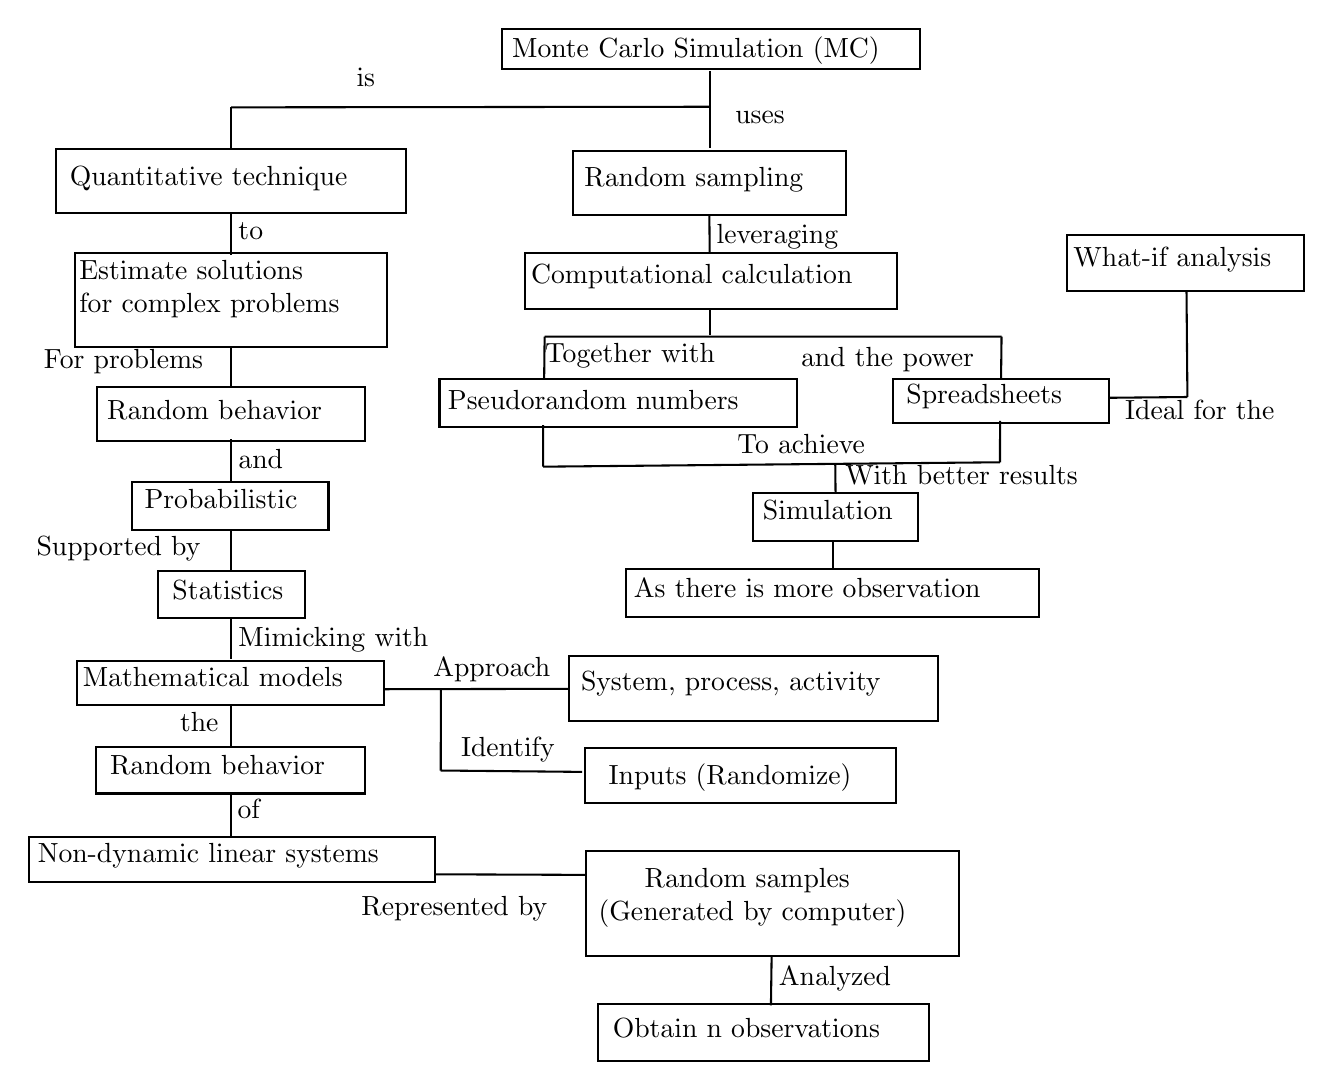
\begin{tikzpicture}[x=0.75pt,y=0.75pt,yscale=-1,xscale=1]
	%uncomment if require: \path (0,533); %set diagram left start at 0, and has height of 533
	
	%Shape: Rectangle [id:dp4215263234124962] 
	\draw   (250.3,22.4) -- (451.7,22.4) -- (451.7,42) -- (250.3,42) -- cycle ;
	
	%Shape: Rectangle [id:dp5605986393419784] 
	\draw   (284.31,81.14) -- (415.64,81.14) -- (415.64,112.05) -- (284.31,112.05) -- cycle ;
	
	%Shape: Rectangle [id:dp6822124988658465] 
	\draw   (35.36,80.38) -- (204.02,80.38) -- (204.02,111.05) -- (35.36,111.05) -- cycle ;
	
	%Straight Lines [id:da24917666653444992] 
	\draw    (119.64,60.29) -- (119.64,80.29) ;
	%Shape: Rectangle [id:dp9161612452597685] 
	\draw   (44.36,130.57) -- (194.5,130.57) -- (194.5,175.71) -- (44.36,175.71) -- cycle ;
	
	%Shape: Rectangle [id:dp8552131257525999] 
	\draw   (54.93,194.86) -- (184.21,194.86) -- (184.21,220.86) -- (54.93,220.86) -- cycle ;
	
	%Shape: Rectangle [id:dp28699352071595885] 
	\draw   (71.79,240.57) -- (166.5,240.57) -- (166.5,264) -- (71.79,264) -- cycle ;
	
	%Shape: Rectangle [id:dp9391104634008505] 
	\draw   (84.36,283.71) -- (155.36,283.71) -- (155.36,306.29) -- (84.36,306.29) -- cycle ;
	
	%Shape: Rectangle [id:dp8058266749569549] 
	\draw   (45.5,326.86) -- (193.07,326.86) -- (193.07,348.29) -- (45.5,348.29) -- cycle ;
	
	%Shape: Rectangle [id:dp6778401923058543] 
	\draw   (54.64,368.29) -- (184.21,368.29) -- (184.21,390.86) -- (54.64,390.86) -- cycle ;
	
	%Shape: Rectangle [id:dp04288092205088323] 
	\draw   (22.07,412) -- (217.64,412) -- (217.64,433.71) -- (22.07,433.71) -- cycle ;
	
	%Straight Lines [id:da42743025398796664] 
	\draw    (119.64,111.29) -- (119.64,131.29) ;
	%Straight Lines [id:da44451579341625] 
	\draw    (119.64,175.29) -- (119.64,195.29) ;
	%Straight Lines [id:da2952815700269025] 
	\draw    (119.64,220.29) -- (119.64,240.29) ;
	%Straight Lines [id:da23583722394609818] 
	\draw    (119.64,264.29) -- (119.64,284.29) ;
	%Straight Lines [id:da8623849950040359] 
	\draw    (119.64,306.29) -- (119.64,326.29) ;
	%Straight Lines [id:da20115540357810247] 
	\draw    (119.64,348.29) -- (119.64,368.29) ;
	%Straight Lines [id:da5844455334116092] 
	\draw    (119.64,391.29) -- (119.64,411.29) ;
	
	%Straight Lines [id:da3223201886985534] 
	\draw    (350.21,42.86) -- (350.21,80) ;
	%Straight Lines [id:da5360135696422039] 
	\draw    (119.64,60.29) -- (350.5,60) ;
	
	%Straight Lines [id:da04617213993490532] 
	\draw    (350,112.21) -- (350.17,130.54) ;
	%Shape: Rectangle [id:dp19377800699756875] 
	\draw   (261.11,130.29) -- (440.33,130.29) -- (440.33,157.62) -- (261.11,157.62) -- cycle ;
	
	%Shape: Rectangle [id:dp9948484136770976] 
	\draw   (220,191.18) -- (392.11,191.18) -- (392.11,214.29) -- (220,214.29) -- cycle ;
	
	%Shape: Rectangle [id:dp3384676720419708] 
	\draw   (438.44,191.18) -- (542.56,191.18) -- (542.56,212.51) -- (438.44,212.51) -- cycle ;
	
	%Shape: Rectangle [id:dp27123736378500474] 
	\draw   (370.89,246.07) -- (450.56,246.07) -- (450.56,269.18) -- (370.89,269.18) -- cycle ;
	
	%Shape: Rectangle [id:dp38853819472250084] 
	\draw   (309.78,282.73) -- (509,282.73) -- (509,305.62) -- (309.78,305.62) -- cycle ;
	
	%Straight Lines [id:da014310810654853512] 
	\draw    (350.22,157.21) -- (350.22,170.14) ;
	%Straight Lines [id:da4776425539155458] 
	\draw    (270.64,170.78) -- (270.41,190.77) ;
	%Straight Lines [id:da4769047517207039] 
	\draw    (270.64,170.78) -- (490.78,170.73) ;
	%Straight Lines [id:da7827579715275725] 
	\draw    (490.78,170.73) -- (490.54,190.72) ;
	%Straight Lines [id:da7330155577088908] 
	\draw    (410.8,245.61) -- (410.67,232.68) ;
	%Straight Lines [id:da8509011957588517] 
	\draw    (490.02,231.29) -- (490.07,211.3) ;
	%Straight Lines [id:da5588878306465803] 
	\draw    (490.02,231.29) -- (269.9,233.41) ;
	%Straight Lines [id:da6769845464898216] 
	\draw    (269.9,233.41) -- (269.94,213.42) ;
	
	%Straight Lines [id:da6666639120422786] 
	\draw    (409.78,269.65) -- (409.78,282.58) ;
	%Shape: Rectangle [id:dp8402670006761139] 
	\draw   (522.44,121.62) -- (636.56,121.62) -- (636.56,148.84) -- (522.44,148.84) -- cycle ;
	
	%Straight Lines [id:da5295493181430606] 
	\draw    (580.33,199.84) -- (542.67,200.22) ;
	%Straight Lines [id:da9855214298674604] 
	\draw    (579.89,148.51) -- (580.33,199.84) ;
	
	%Shape: Rectangle [id:dp5002143400150245] 
	\draw   (282.33,324.46) -- (460,324.46) -- (460,355.8) -- (282.33,355.8) -- cycle ;
	
	%Shape: Rectangle [id:dp35257179506306247] 
	\draw   (290,369.13) -- (440,369.13) -- (440,395.46) -- (290,395.46) -- cycle ;
	
	%Shape: Rectangle [id:dp4882311664786725] 
	\draw   (290.43,418.65) -- (470.1,418.65) -- (470.1,469.32) -- (290.43,469.32) -- cycle ;
	
	%Shape: Rectangle [id:dp0619736638622812] 
	\draw   (296.33,492.46) -- (456,492.46) -- (456,519.8) -- (296.33,519.8) -- cycle ;
	
	%Straight Lines [id:da8550561367501606] 
	\draw    (193.33,340.63) -- (281.86,340.44) ;
	%Straight Lines [id:da39616791435448273] 
	\draw    (220.57,379.8) -- (288.67,380.46) ;
	%Straight Lines [id:da11167548719220122] 
	\draw    (220.67,340.55) -- (220.57,379.8) ;
	%Straight Lines [id:da16209257991496884] 
	\draw    (217.71,429.8) -- (290.71,430.08) ;
	%Straight Lines [id:da46148840186933593] 
	\draw    (380,469.55) -- (379.67,492.94) ;
	
	% Text Node
	\draw (253.5,25) node [anchor=north west][inner sep=0.75pt]   [align=left] {Monte Carlo Simulation (MC)};
	% Text Node
	\draw (288.31,87.79) node [anchor=north west][inner sep=0.75pt]   [align=left] {Random sampling};
	% Text Node
	\draw (40.36,87.38) node [anchor=north west][inner sep=0.75pt]   [align=left] {Quantitative technique};
	% Text Node
	\draw (44.93,132.43) node [anchor=north west][inner sep=0.75pt]   [align=left] {Estimate solutions \\for complex problems};
	% Text Node
	\draw (58.36,199.86) node [anchor=north west][inner sep=0.75pt]   [align=left] {Random behavior};
	% Text Node
	\draw (76.36,242.86) node [anchor=north west][inner sep=0.75pt]   [align=left] {Probabilistic};
	% Text Node
	\draw (89.79,286.86) node [anchor=north west][inner sep=0.75pt]   [align=left] {Statistics};
	% Text Node
	\draw (46.64,328.43) node [anchor=north west][inner sep=0.75pt]   [align=left] {Mathematical models};
	% Text Node
	\draw (59.79,370.86) node [anchor=north west][inner sep=0.75pt]   [align=left] {Random behavior};
	% Text Node
	\draw (24.93,413.57) node [anchor=north west][inner sep=0.75pt]   [align=left] {Non-dynamic linear systems};
	% Text Node
	\draw (178.5,40) node [anchor=north west][inner sep=0.75pt]   [align=left] {is};
	% Text Node
	\draw (361,61) node [anchor=north west][inner sep=0.75pt]   [align=left] {uses};
	% Text Node
	\draw (121.64,114.29) node [anchor=north west][inner sep=0.75pt]   [align=left] {to};
	% Text Node
	\draw (27.93,175.21) node [anchor=north west][inner sep=0.75pt]   [align=left] {For problems};
	% Text Node
	\draw (121.64,223.29) node [anchor=north west][inner sep=0.75pt]   [align=left] {and};
	% Text Node
	\draw (24.36,265.29) node [anchor=north west][inner sep=0.75pt]   [align=left] {Supported by};
	% Text Node
	\draw (121.64,309.29) node [anchor=north west][inner sep=0.75pt]   [align=left] {Mimicking with};
	% Text Node
	\draw (93.5,350.43) node [anchor=north west][inner sep=0.75pt]   [align=left] {the};
	% Text Node
	\draw (121.21,392.14) node [anchor=north west][inner sep=0.75pt]   [align=left] {of};
	% Text Node
	\draw (262.61,134.61) node [anchor=north west][inner sep=0.75pt]   [align=left] {Computational calculation};
	% Text Node
	\draw (222.56,195.22) node [anchor=north west][inner sep=0.75pt]   [align=left] {Pseudorandom numbers};
	% Text Node
	\draw (374.33,247.94) node [anchor=north west][inner sep=0.75pt]   [align=left] {Simulation};
	% Text Node
	\draw (312.17,285.67) node [anchor=north west][inner sep=0.75pt]   [align=left] {As there is more observation};
	% Text Node
	\draw (443.44,192.44) node [anchor=north west][inner sep=0.75pt]   [align=left] {Spreadsheets};
	% Text Node
	\draw (523.94,126.06) node [anchor=north west][inner sep=0.75pt]   [align=left] {What-if analysis};
	% Text Node
	\draw (286.67,330.62) node [anchor=north west][inner sep=0.75pt]   [align=left] {System, process, activity};
	% Text Node
	\draw (300,374.95) node [anchor=north west][inner sep=0.75pt]   [align=left] {Inputs (Randomize)};
	% Text Node
	\draw (295.1,425.48) node [anchor=north west][inner sep=0.75pt]   [align=left] { \ \ \ \ \ Random samples \\(Generated by computer)};
	% Text Node
	\draw (302,497.62) node [anchor=north west][inner sep=0.75pt]   [align=left] {Obtain n observations};
	% Text Node
	\draw (352,115.21) node [anchor=north west][inner sep=0.75pt]   [align=left] {leveraging};
	% Text Node
	\draw (269.33,172.67) node [anchor=north west][inner sep=0.75pt]   [align=left] {Together with};
	% Text Node
	\draw (392.67,174.33) node [anchor=north west][inner sep=0.75pt]   [align=left] {and the power};
	% Text Node
	\draw (362,216.33) node [anchor=north west][inner sep=0.75pt]   [align=left] {To achieve};
	% Text Node
	\draw (414,231.33) node [anchor=north west][inner sep=0.75pt]   [align=left] {With better results};
	% Text Node
	\draw (215.52,323.76) node [anchor=north west][inner sep=0.75pt]   [align=left] {Approach};
	% Text Node
	\draw (228.86,362.16) node [anchor=north west][inner sep=0.75pt]   [align=left] {Identify};
	% Text Node
	\draw (180.86,438.87) node [anchor=north west][inner sep=0.75pt]   [align=left] {Represented by};
	% Text Node
	\draw (382,472.55) node [anchor=north west][inner sep=0.75pt]   [align=left] {Analyzed};
	% Text Node
	\draw (548.86,199.73) node [anchor=north west][inner sep=0.75pt]   [align=left] {Ideal for the};
	
	
\end{tikzpicture}
\end{adjustbox}
\end{center}


El algoritmo de monte carlo utilizará como función objetivo la menor cantidad de movimientos para poder ganar la partida. No obstante, también se hará uso de una heurística, esto porque aparte de guiar el camino para la solución; como muy probablemente el árbol no pueda llegar a simular hasta tener el coste total, entonces la heurística al ser optimista llevará por caminos según su propiedad. 

\(h1(n)\) = Puntaje del jugador en base al valor de cada pieza.\\

\(c\) = Coste (Cantidad de jugadas hasta el jaque mate)

\begin{enumerate}
	\item \textbf{Admisibilidad}: La heurística resulta admisible porque relaja el problema. Ya no busca realizar jaque mate que puede resultar complejo, comenzará a buscar la mayor puntuación que implica solo comer las más valiosas posibles
	\item \textbf{Consistencia}: Es consistente, porque conforme se tengan más sucesores, estos siempre resultan más sencillos debido a la cantidad de puntaje reducido.
\end{enumerate}

En base a lo que pueda jugar el algoritmo, se le pondrá como contrincante otro igual para que así simulen partidas; y como el algoritmo buscará el mejor movimiento posible, entonces de esta manera se nos proveerá de data útil para la red neuronal, cosa que realizando partidas con personas resultaría tanto más costoso, como no necesariamente valioso, porque estas personas pueden cometer errores. Se simularán aproximadamente cien partidas, para a partir de aquí guardar en un dataset tanto entradas como salidas que resultarán de aprendizaje para la red neuronal.

\subsection{Dataset}
El dataset que se genere a partir de las partidas de Monte Carlo, consistirá en dos vectores. El primero será el tablero de ajedrez que tendrá identificada cada pieza con un número y un signo.

\begin{tabular}{|c|c|c|c|c|}
	\hline
	\textbf{Pieza} & \textbf{ID} & \textbf{Blanco} & \textbf{Negro} & \textbf{Valor} \\ \hline
	Torre 1 & 1 & 1 & -1 & $1 \times \text{Color}$ \\ \hline
	Caballo 1 & 2 & 1 & -1 & $2 \times \text{Color}$ \\ \hline
	Alfil 1 & 3 & 1 & -1 & $3 \times \text{Color}$ \\ \hline
	Reina & 4 & 1 & -1 & $4 \times \text{Color}$ \\ \hline
	Rey & 5 & 1 & -1 & $5 \times \text{Color}$ \\ \hline
	Alfil 2 & 6 & 1 & -1 & $6 \times \text{Color}$ \\ \hline
	Caballo 2 & 7 & 1 & -1 & $7 \times \text{Color}$ \\ \hline
	Torre 2 & 8 & 1 & -1 & $8 \times \text{Color}$ \\ \hline
	Peon & [9...16] & 1 & -1 & $i \times \text{Color}$ \\ \hline
	Vacio & 0 & 0 & 0 & 0 \\ \hline
\end{tabular}

Y con estos valores, el tablero que se tenga en base a strings se convertirá en un arreglo numérico basado en el diccionario previamente establecido.
Con respecto al output para predecir, se utilizará de igual manera un vector. Este indicará:

v = (Movimiento, Origen 1, Origen 2, Destino 1, Destino 2, Coronación)

Y los valores establecidos para cada uno de los parámetros del vector son:

\subsubsection{Movimiento}
\begin{center}
	\begin{tabular}{|c|c|}
		\hline
		\textbf{Movimiento} & \textbf{Valor} \\ \hline
		Basico & 1\\ \hline
		Split  & 2 \\\hline
		Swap   & 3 \\\hline
	\end{tabular}
\end{center}
Para el movimiento no se toma en cuenta el slide, ya que, está implícito dentro de cualquier movimiento, menos el merge.

\subsubsection{Orígenes y destinos}
\begin{center}
	\begin{tabular}{|c|c|c|}
		\hline
		\textbf{Valor} & \textbf{Necesita movimiento} & \textbf{No necesita} \\ \hline
		Origen 1    & [ 0,63 ] & -\\ \hline
		Origen 2    & [ 0,63 ] & -1\\\hline
		Destino 1   & [ 0,63 ] & -\\\hline
		Destino 2   & [ 0,63 ] & -1\\\hline
	\end{tabular}
\end{center}
\subsubsection{Coronación}
\begin{center}
	\begin{tabular}{|c|c|}
		\hline
		\textbf{Pieza} & \textbf{Valor} \\ \hline
		Reina & 0\\ \hline
		Torre  & 1 \\\hline
		Caballo   & 2 \\\hline
		Alfil   & 3 \\\hline
		No hay   & -1 \\\hline
	\end{tabular}    
\end{center}

La data no llevará un tratamiento especial, ya que, como es generada por el computador, esta ya está completa y es fiable por el algoritmo que la generó

\subsection{Multi Layer Neural Network}
Encargado de tomar las desiciones en base de los  analisis realizados a nivel del Montecarlo. Es el  responsable de ordenar que es lo que se hace mientras avanza la partida de ajedrez que busca ganar el algoritmo.\newline
Tras conseguir de las simulaciones con Monte Carlo data de entrenamiento. Esta se procederá a utilizar como input a la red neuronal.\newline
Para el proceso de entrenamiento se tomará a la data con un 25\% que será para el test, mientras que un 75\% para el train. De esta forma se podrá ver si las jugadas que realizará el modelo tienen lógica con lo que aprendió y si realmente está trabajando bajo la misma lógica de Monte Carlo para llegar a las mismas conclusiones sobre qué movimientos realizar.\newline
La red neuronal multicapa se encargará de mejorar el proceso de aprendizaje, ya que, pasará por capas de neuronas, para así ajustar a cada parámetro de salida necesario de manera más óptima. De igual manera habrá una capa final que ajustará los resultados a la salida que realmente sirve, ya que, lo que se plantea predecir es discreto dentro de rangos fijos según cada componente.\newline
La cantidad de capas o la cantidad de neuronas por capas, y todos los hiper parámetros, se inicializará según la bibliografía estudiada, pero se irán ajustando con el uso del Bat Algorithm.\newline
Finalmente, cuando se compruebe que la red puede predecir movimientos del algoritmo Monte Carlo, entonces se pondrá a prueba en juegos para ver su funcionamiento.

\subsection{Bat Algorithm}
Si bien debido al dataset generado de manera confiable gracias al Monte Carlo Tree Search, de todas formas, se deben de optimizar los hiper parámetros de las redes neuronales. Para esta optimización se utilizará el bat algorithm.

%PEUSODCÓDIGO BAT ALGORITHm
\begin{center}
\begin{adjustbox}{width=7cm, height=12cm, keepaspectratio}
\tikzset{every picture/.style={line width=0.75pt}} %set default line width to 0.75pt        

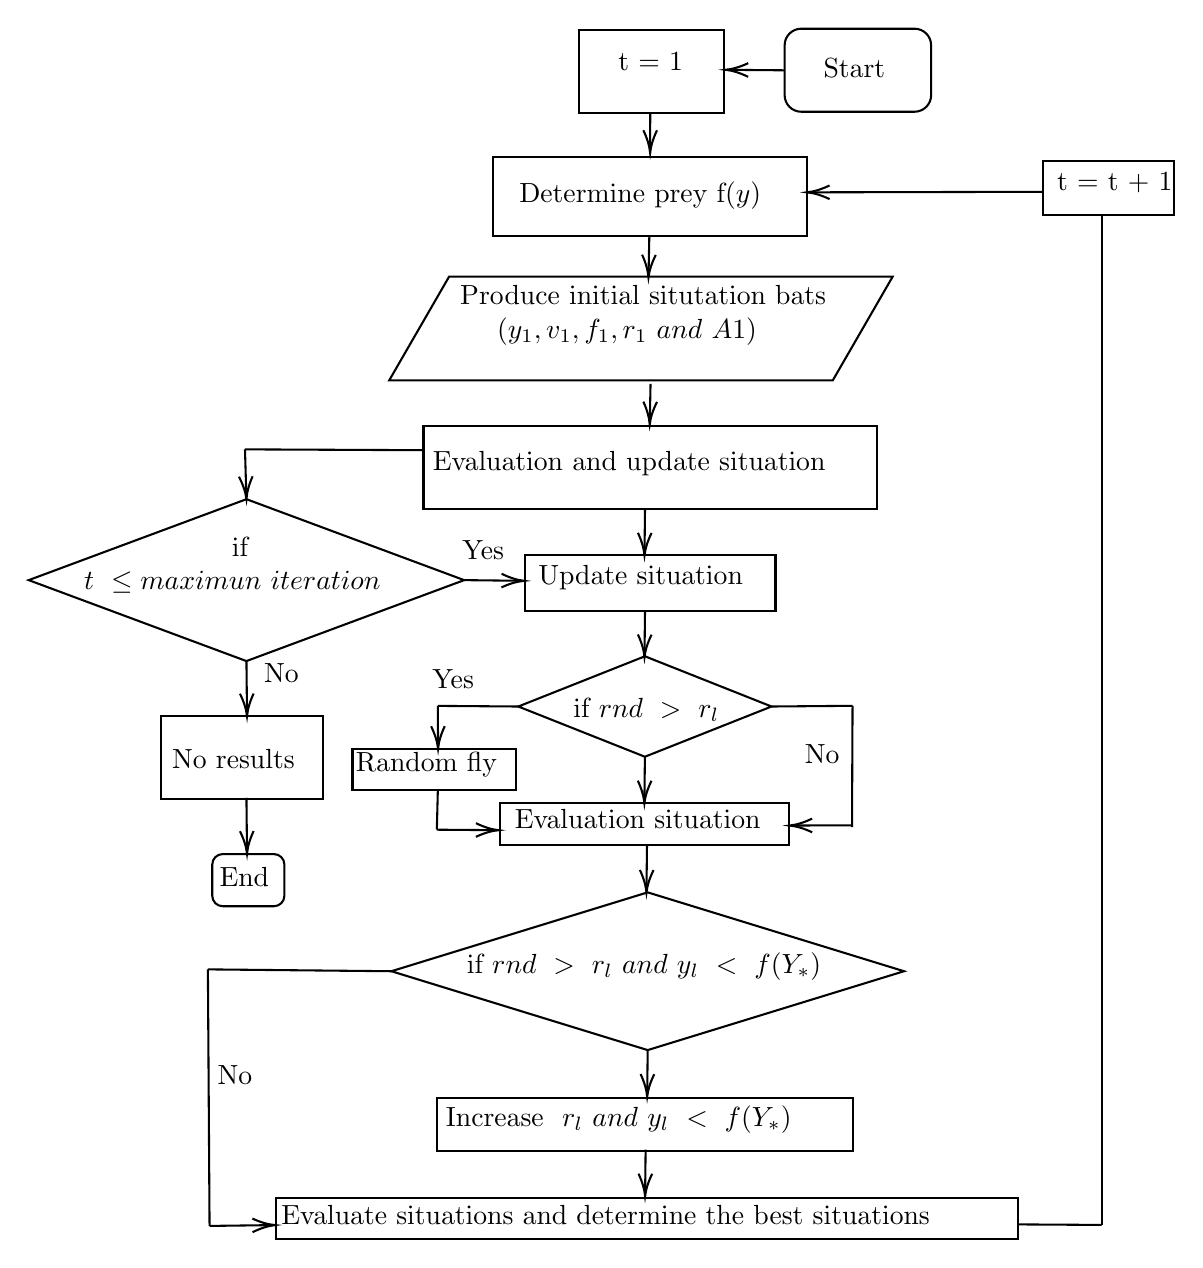
\begin{tikzpicture}[x=0.75pt,y=0.75pt,yscale=-1,xscale=1]
	%uncomment if require: \path (0,1122); %set diagram left start at 0, and has height of 1122
	
	%Shape: Rectangle [id:dp11199231081600236] 
	\draw   (288.02,34.47) -- (358.02,34.47) -- (358.02,74.47) -- (288.02,74.47) -- cycle ;
	
	%Shape: Rectangle [id:dp9862949515841928] 
	\draw   (246.6,95.5) -- (397.93,95.5) -- (397.93,133.67) -- (246.6,133.67) -- cycle ;
	
	%Rounded Rect [id:dp8968724601667921] 
	\draw   (387.27,41.8) .. controls (387.27,37.38) and (390.85,33.8) .. (395.27,33.8) -- (449.85,33.8) .. controls (454.27,33.8) and (457.85,37.38) .. (457.85,41.8) -- (457.85,65.8) .. controls (457.85,70.22) and (454.27,73.8) .. (449.85,73.8) -- (395.27,73.8) .. controls (390.85,73.8) and (387.27,70.22) .. (387.27,65.8) -- cycle ;
	
	%Straight Lines [id:da1448631814999326] 
	\draw    (387.02,53.84) -- (360.77,53.61) ;
	\draw [shift={(358.77,53.59)}, rotate = 0.51] [color={rgb, 255:red, 0; green, 0; blue, 0 }  ][line width=0.75]    (10.93,-3.29) .. controls (6.95,-1.4) and (3.31,-0.3) .. (0,0) .. controls (3.31,0.3) and (6.95,1.4) .. (10.93,3.29)   ;
	%Straight Lines [id:da08995180587744223] 
	\draw    (322.52,74.09) -- (322.47,91.67) ;
	\draw [shift={(322.47,93.67)}, rotate = 270.15] [color={rgb, 255:red, 0; green, 0; blue, 0 }  ][line width=0.75]    (10.93,-3.29) .. controls (6.95,-1.4) and (3.31,-0.3) .. (0,0) .. controls (3.31,0.3) and (6.95,1.4) .. (10.93,3.29)   ;
	%Shape: Rectangle [id:dp11994357769035191] 
	\draw   (225.6,153.27) -- (439.31,153.27) -- (410.44,203.27) -- (196.73,203.27) -- cycle ;
	
	%Shape: Rectangle [id:dp6991932005539763] 
	\draw   (213.27,225.07) -- (431.67,225.07) -- (431.67,265.07) -- (213.27,265.07) -- cycle ;
	
	%Straight Lines [id:da5570849935229241] 
	\draw    (322.07,134.07) -- (321.71,151.67) ;
	\draw [shift={(321.67,153.67)}, rotate = 271.17] [color={rgb, 255:red, 0; green, 0; blue, 0 }  ][line width=0.75]    (10.93,-3.29) .. controls (6.95,-1.4) and (3.31,-0.3) .. (0,0) .. controls (3.31,0.3) and (6.95,1.4) .. (10.93,3.29)   ;
	%Straight Lines [id:da23972455000161563] 
	\draw    (322.67,204.87) -- (322.31,222.47) ;
	\draw [shift={(322.27,224.47)}, rotate = 271.17] [color={rgb, 255:red, 0; green, 0; blue, 0 }  ][line width=0.75]    (10.93,-3.29) .. controls (6.95,-1.4) and (3.31,-0.3) .. (0,0) .. controls (3.31,0.3) and (6.95,1.4) .. (10.93,3.29)   ;
	
	%Shape: Rectangle [id:dp3372630993033694] 
	\draw   (262.07,287.27) -- (382.87,287.27) -- (382.87,314.21) -- (262.07,314.21) -- cycle ;
	
	%Shape: Diamond [id:dp22966171081387388] 
	\draw   (127.97,260.47) -- (232.87,299.47) -- (127.97,338.47) -- (23.07,299.47) -- cycle ;
	
	%Straight Lines [id:da2896807914403723] 
	\draw    (127.27,236.47) -- (213.27,236.87) ;
	%Straight Lines [id:da15189665526347684] 
	\draw    (127.27,236.47) -- (127.91,258.47) ;
	\draw [shift={(127.97,260.47)}, rotate = 268.33] [color={rgb, 255:red, 0; green, 0; blue, 0 }  ][line width=0.75]    (10.93,-3.29) .. controls (6.95,-1.4) and (3.31,-0.3) .. (0,0) .. controls (3.31,0.3) and (6.95,1.4) .. (10.93,3.29)   ;
	%Shape: Rectangle [id:dp751137217740556] 
	\draw   (87,364.88) -- (165,364.88) -- (165,404.88) -- (87,404.88) -- cycle ;
	%Straight Lines [id:da5722635336416755] 
	\draw    (127.97,338.07) -- (128.23,363.08) ;
	\draw [shift={(128.25,365.08)}, rotate = 269.4] [color={rgb, 255:red, 0; green, 0; blue, 0 }  ][line width=0.75]    (10.93,-3.29) .. controls (6.95,-1.4) and (3.31,-0.3) .. (0,0) .. controls (3.31,0.3) and (6.95,1.4) .. (10.93,3.29)   ;
	%Rounded Rect [id:dp3776201245469004] 
	\draw   (111.5,436.48) .. controls (111.5,433.71) and (113.75,431.46) .. (116.52,431.46) -- (141.22,431.46) .. controls (144,431.46) and (146.25,433.71) .. (146.25,436.48) -- (146.25,451.56) .. controls (146.25,454.33) and (144,456.58) .. (141.22,456.58) -- (116.52,456.58) .. controls (113.75,456.58) and (111.5,454.33) .. (111.5,451.56) -- cycle ;
	%Straight Lines [id:da8638079389758646] 
	\draw    (127.97,404.32) -- (128.23,429.33) ;
	\draw [shift={(128.25,431.33)}, rotate = 269.4] [color={rgb, 255:red, 0; green, 0; blue, 0 }  ][line width=0.75]    (10.93,-3.29) .. controls (6.95,-1.4) and (3.31,-0.3) .. (0,0) .. controls (3.31,0.3) and (6.95,1.4) .. (10.93,3.29)   ;
	%Straight Lines [id:da11071951771999644] 
	\draw    (232.87,299.47) -- (259.8,299.78) ;
	\draw [shift={(261.8,299.81)}, rotate = 180.67] [color={rgb, 255:red, 0; green, 0; blue, 0 }  ][line width=0.75]    (10.93,-3.29) .. controls (6.95,-1.4) and (3.31,-0.3) .. (0,0) .. controls (3.31,0.3) and (6.95,1.4) .. (10.93,3.29)   ;
	%Shape: Rectangle [id:dp7677856775494443] 
	\draw   (511.75,97.75) -- (574.74,97.75) -- (574.74,123.38) -- (511.75,123.38) -- cycle ;
	
	%Flowchart: Decision [id:dp8703229913913602] 
	\draw   (319.95,336.16) -- (380.95,360.36) -- (319.95,384.56) -- (258.95,360.36) -- cycle ;
	
	%Straight Lines [id:da9178130710975352] 
	\draw    (320,265.13) -- (319.77,285.63) ;
	\draw [shift={(319.75,287.63)}, rotate = 270.64] [color={rgb, 255:red, 0; green, 0; blue, 0 }  ][line width=0.75]    (10.93,-3.29) .. controls (6.95,-1.4) and (3.31,-0.3) .. (0,0) .. controls (3.31,0.3) and (6.95,1.4) .. (10.93,3.29)   ;
	%Straight Lines [id:da2314187329435875] 
	\draw    (320,314.13) -- (319.77,334.63) ;
	\draw [shift={(319.75,336.63)}, rotate = 270.64] [color={rgb, 255:red, 0; green, 0; blue, 0 }  ][line width=0.75]    (10.93,-3.29) .. controls (6.95,-1.4) and (3.31,-0.3) .. (0,0) .. controls (3.31,0.3) and (6.95,1.4) .. (10.93,3.29)   ;
	%Shape: Rectangle [id:dp6582185527266435] 
	\draw   (250,406.63) -- (389.25,406.63) -- (389.25,427.13) -- (250,427.13) -- cycle ;
	
	%Straight Lines [id:da34391865470559635] 
	\draw    (319.95,384.56) -- (319.72,405.06) ;
	\draw [shift={(319.7,407.06)}, rotate = 270.64] [color={rgb, 255:red, 0; green, 0; blue, 0 }  ][line width=0.75]    (10.93,-3.29) .. controls (6.95,-1.4) and (3.31,-0.3) .. (0,0) .. controls (3.31,0.3) and (6.95,1.4) .. (10.93,3.29)   ;
	%Straight Lines [id:da652495846083273] 
	\draw    (380.95,360.36) -- (419.99,360.02) ;
	%Straight Lines [id:da897182143286203] 
	\draw    (419.99,360.02) -- (419.87,386.54) -- (419.74,418.44) ;
	%Straight Lines [id:da46603224656077225] 
	\draw    (419.59,417.59) -- (391.59,417.7) ;
	\draw [shift={(389.59,417.71)}, rotate = 359.78] [color={rgb, 255:red, 0; green, 0; blue, 0 }  ][line width=0.75]    (10.93,-3.29) .. controls (6.95,-1.4) and (3.31,-0.3) .. (0,0) .. controls (3.31,0.3) and (6.95,1.4) .. (10.93,3.29)   ;
	%Shape: Rectangle [id:dp17603542487610757] 
	\draw   (179.06,380.89) -- (257.94,380.89) -- (257.94,400.77) -- (179.06,400.77) -- cycle ;
	
	%Straight Lines [id:da9914039358654374] 
	\draw    (220.18,360.06) -- (258.95,360.36) ;
	%Straight Lines [id:da845517841725834] 
	\draw    (220.18,360.06) -- (220.28,378.77) ;
	\draw [shift={(220.29,380.77)}, rotate = 269.67] [color={rgb, 255:red, 0; green, 0; blue, 0 }  ][line width=0.75]    (10.93,-3.29) .. controls (6.95,-1.4) and (3.31,-0.3) .. (0,0) .. controls (3.31,0.3) and (6.95,1.4) .. (10.93,3.29)   ;
	%Straight Lines [id:da8026235885310966] 
	\draw    (219.71,419.71) -- (247.47,419.93) ;
	\draw [shift={(249.47,419.95)}, rotate = 180.45] [color={rgb, 255:red, 0; green, 0; blue, 0 }  ][line width=0.75]    (10.93,-3.29) .. controls (6.95,-1.4) and (3.31,-0.3) .. (0,0) .. controls (3.31,0.3) and (6.95,1.4) .. (10.93,3.29)   ;
	%Straight Lines [id:da4698634035103251] 
	\draw    (220.18,400.77) -- (219.71,419.71) ;
	%Flowchart: Decision [id:dp5319849058371844] 
	\draw   (321.29,449.9) -- (444.79,487.9) -- (321.29,525.9) -- (197.79,487.9) -- cycle ;
	
	%Straight Lines [id:da49738942927815155] 
	\draw    (320.95,427.56) -- (320.72,448.06) ;
	\draw [shift={(320.7,450.06)}, rotate = 270.64] [color={rgb, 255:red, 0; green, 0; blue, 0 }  ][line width=0.75]    (10.93,-3.29) .. controls (6.95,-1.4) and (3.31,-0.3) .. (0,0) .. controls (3.31,0.3) and (6.95,1.4) .. (10.93,3.29)   ;
	%Shape: Rectangle [id:dp5910651871448562] 
	\draw   (219.71,549.01) -- (420.14,549.01) -- (420.14,574.44) -- (219.71,574.44) -- cycle ;
	
	%Straight Lines [id:da6793033065905993] 
	\draw    (321.29,525.9) -- (321.06,546.4) ;
	\draw [shift={(321.04,548.4)}, rotate = 270.64] [color={rgb, 255:red, 0; green, 0; blue, 0 }  ][line width=0.75]    (10.93,-3.29) .. controls (6.95,-1.4) and (3.31,-0.3) .. (0,0) .. controls (3.31,0.3) and (6.95,1.4) .. (10.93,3.29)   ;
	%Shape: Rectangle [id:dp11865248416776497] 
	\draw   (142,597.01) -- (499.8,597.01) -- (499.8,617.01) -- (142,617.01) -- cycle ;
	
	%Straight Lines [id:da715318697506399] 
	\draw    (320.29,573.9) -- (320.06,594.4) ;
	\draw [shift={(320.04,596.4)}, rotate = 270.64] [color={rgb, 255:red, 0; green, 0; blue, 0 }  ][line width=0.75]    (10.93,-3.29) .. controls (6.95,-1.4) and (3.31,-0.3) .. (0,0) .. controls (3.31,0.3) and (6.95,1.4) .. (10.93,3.29)   ;
	%Straight Lines [id:da07560498995790077] 
	\draw    (197.79,487.9) -- (109.4,487.01) ;
	%Straight Lines [id:da7580180842113537] 
	\draw    (109.4,487.01) -- (110.2,610.61) ;
	%Straight Lines [id:da8516305823196955] 
	\draw    (110.2,610.61) -- (139.8,610.23) ;
	\draw [shift={(141.8,610.21)}, rotate = 179.27] [color={rgb, 255:red, 0; green, 0; blue, 0 }  ][line width=0.75]    (10.93,-3.29) .. controls (6.95,-1.4) and (3.31,-0.3) .. (0,0) .. controls (3.31,0.3) and (6.95,1.4) .. (10.93,3.29)   ;
	%Straight Lines [id:da3647469968746617] 
	\draw    (540,610.13) -- (540,123.13) ;
	%Straight Lines [id:da12968082436596862] 
	\draw    (540,610.13) -- (500,609.88) ;
	%Straight Lines [id:da5098312321281846] 
	\draw    (511.5,112.38) -- (400,112.63) ;
	\draw [shift={(398,112.63)}, rotate = 359.87] [color={rgb, 255:red, 0; green, 0; blue, 0 }  ][line width=0.75]    (10.93,-3.29) .. controls (6.95,-1.4) and (3.31,-0.3) .. (0,0) .. controls (3.31,0.3) and (6.95,1.4) .. (10.93,3.29)   ;
	
	% Text Node
	\draw (305.68,43.63) node [anchor=north west][inner sep=0.75pt]   [align=left] {t = 1};
	% Text Node
	\draw (257.93,106.22) node [anchor=north west][inner sep=0.75pt]   [align=left] {Determine prey f($\displaystyle y)$};
	% Text Node
	\draw (404.55,46.8) node [anchor=north west][inner sep=0.75pt]   [align=left] {Start};
	% Text Node
	\draw (229.47,156.07) node [anchor=north west][inner sep=0.75pt]   [align=left] {Produce initial situtation bats\\\ \ \ \  $\displaystyle ( y_{1} ,v_{1} ,f_{1} ,r_{1} \ and\ A1)$};
	% Text Node
	\draw (216.27,235.67) node [anchor=north west][inner sep=0.75pt]   [align=left] {Evaluation and update situation};
	% Text Node
	\draw (267.07,290.82) node [anchor=north west][inner sep=0.75pt]   [align=left] {Update situation};
	% Text Node
	\draw (43.87,270.47) node [anchor=north west][inner sep=0.75pt]   [align=left] {\\ \ \ \ \ \ \ \ \ \ \ \ \ \ \ \ \ \ if\\ $\displaystyle \ t\ \leq maximun\ iteration$};
	% Text Node
	\draw (90.67,379.54) node [anchor=north west][inner sep=0.75pt]   [align=left] {No results};
	% Text Node
	\draw (113.5,436.21) node [anchor=north west][inner sep=0.75pt]   [align=left] {End};
	% Text Node
	\draw (279.55,348.16) node [anchor=north west][inner sep=0.75pt]   [align=left] {\\ \ if $\displaystyle rnd\  >\ r_{l}$};
	% Text Node
	\draw (255.75,408.51) node [anchor=north west][inner sep=0.75pt]   [align=left] {Evaluation situation};
	% Text Node
	\draw (179.18,380.74) node [anchor=north west][inner sep=0.75pt]   [align=left] {Random fly};
	% Text Node
	\draw (216,341.01) node [anchor=north west][inner sep=0.75pt]   [align=left] {Yes};
	% Text Node
	\draw (230.5,279.01) node [anchor=north west][inner sep=0.75pt]   [align=left] {Yes};
	% Text Node
	\draw (135,338.01) node [anchor=north west][inner sep=0.75pt]   [align=left] {No};
	% Text Node
	\draw (395.5,377.01) node [anchor=north west][inner sep=0.75pt]   [align=left] {No};
	% Text Node
	\draw (223.79,477.65) node [anchor=north west][inner sep=0.75pt]   [align=left] {\ \ if $\displaystyle rnd\  >\ r_{l} \ and\ y_{l} \ < \ f( Y_{*})$};
	% Text Node
	\draw (222.57,551.29) node [anchor=north west][inner sep=0.75pt]   [align=left] {Increase \ $\displaystyle r_{l} \ and\ y_{l} \ < \ f( Y_{*})$ };
	% Text Node
	\draw (143.31,599.24) node [anchor=north west][inner sep=0.75pt]   [align=left] {Evaluate situations and determine the best situations};
	% Text Node
	\draw (112.6,532.01) node [anchor=north west][inner sep=0.75pt]   [align=left] {No};
	% Text Node
	\draw (517.04,101.85) node [anchor=north west][inner sep=0.75pt]   [align=left] {t = t + 1};	
\end{tikzpicture}
\end{adjustbox}
\end{center}


Se basa en la ecolocalización de los murciélagos para así poder llegar a la solución más óptima, en este caso sería la cantidad de capas, las neuronas por capa, la cantidad de épocas, entre otras.

\subsection{Despliegue}

El uso de la red neuronal será únicamente sus pesos para poder predecir a partir de un tablero dado, que movimiento realizar. Para esto, se realizará un despliegue dentro de python para que se pueda jugar con un tablero en ASCII; la metodología de juego será por turnos donde empezará el jugador con las blancas, y la red neuronal será las negras.

